% =======================================================================================
\section{Flow in Relative Coordinates}
\label{sec:flow}\label{sec:method}
% =======================================================================================
% 2026-11-22 (user): the former Method section is split into this section and sec:architecture.

We train one conditional generative model of the window posterior $p(\Theta_w\mid y,\fw)$ of
\cref{eq:gw-factorisation} over all windows of a band. A loud source's posterior is decades
narrower than its prior and a quiet source's is the prior, so no absolute scale suits both, and
the flow works in relative quantities throughout. Its coordinates are relative to the window and
its noise, and carry none of the posterior's symmetries (\cref{sec:method-chart}). Its variable
is relative to a Gaussian frame that the network reads off the data (\cref{sec:method-frame}).
Its loss measures each error relative to the spread the data leave (\cref{sec:method-fm}).
\Cref{sec:architecture} describes the network and its training.

% 2026-11-22 (user): Figure 4 placed here so that it lands on page 6.
\begin{figure*}[t]
  \centering
  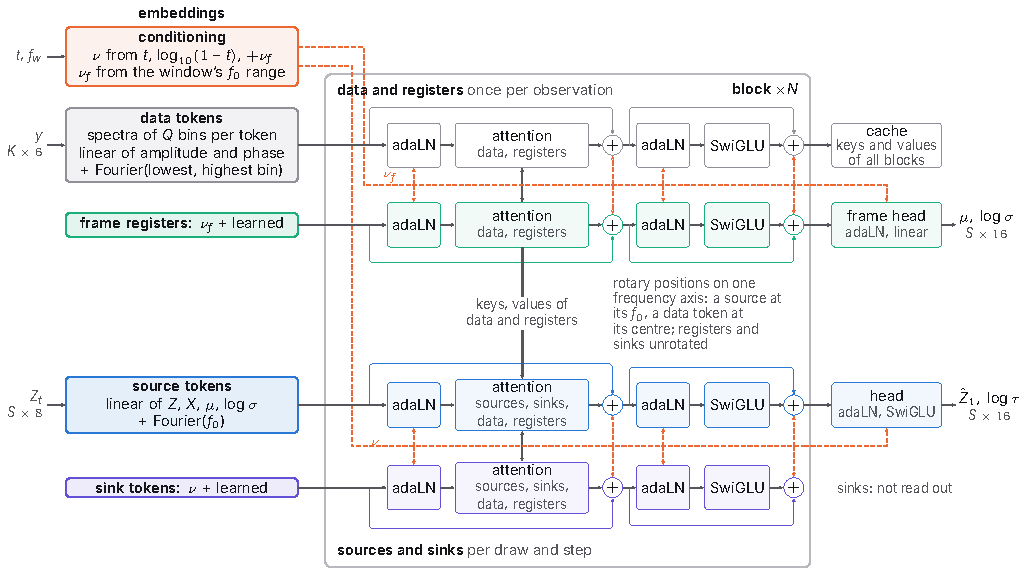
\includegraphics[width=\textwidth]{figures/architecture.pdf}
  \caption{The network: four streams, each with its own normalisations, attention projections and
  feed-forward. The source stream (blue) has one token per source slot, in order of $f_0$, and the
  sink stream (violet) \NetworkSinksWord{} tokens; they attend jointly. The data stream (grey) has
  one token per \NetworkPatch{} frequency bins of the window, and the register stream (green) one
  frame register per slot, which the frame head reads; they attend jointly. Conditioning (orange, dashed) modulates every normalisation and residual gate:
  $\nu$ from the flow time and the window in the source stream and head, $\nu_f$ from the window
  alone in the data stream, the registers and the frame head. The data side never reads the
  sources, so its keys and values and the frame are computed once per observation and serve every
  draw and sampler step. Rotary positions place each source at its $f_0$ and each data token at its
  centre frequency.}
  \label{fig:network-architecture}
\end{figure*}

\subsection{Coordinates Relative to the Window}
\label{sec:method-chart}\label{sec:gw-chart}

The likelihood is invariant under $(\psi,\phi_0)\to(\psi+\pi/2,\phi_0+\pi)$, which gives each source
four copies in $(\psi,\phi_0)\in[0,2\pi)^2$ (\cref{eq:psi-phi-symmetry}), and under the $S!$
permutations of the sources. A posterior over the physical parameters therefore has $4^S\,S!$
equivalent modes, and a flow on them must put mass on every one. The velocity that flow matching
regresses is then an average over the copies for much of the path, which washes out the phase.

The flow draws $X\in\R^{8S}$, eight coordinates per source (\cref{eq:chart}). The frequency is
scaled to the window, $\log\fdot$ is standardised given $f_0$, and the sky is in galactic
coordinates scaled by the prior's widths. In place of amplitude, inclination, polarisation and
phase the source carries its two complex helicity amplitudes, in units of the noise at the window
centre and with the radius warped by $\operatorname{asinh}$,
\begin{equation}
\begin{aligned}
  \zeta_\pm &= \frac{\Amp}{u(\fw)}\,\frac{(1\mp\cos\iota)^2}{4}\,e^{\ii(\phi_0^{\rm mid}\pm2\psi)},\\
  z_\pm &= \operatorname{asinh}\lvert\zeta_\pm\rvert\;\frac{\zeta_\pm}{\lvert\zeta_\pm\rvert},
\end{aligned}
  \label{eq:chart-helicity}
\end{equation}
where $u(\fw)$ is the noise amplitude at the window centre (\cref{app:chart-unit}) and
$\phi_0^{\rm mid}$ the phase referred to mid-observation (\cref{eq:chart-phase}). The sources occupy
$S$ slots in order of $f_0$, the ordering cure for label switching
\citep{stephens2000dealing,jasra2005markov,buscicchio2019label} that the global fit also uses
\citep{littenberg2020global}.

The signal is linear in $\zeta_\pm$ (\cref{eq:forward-model-helicity}), so at fixed frequency, drift
and sky the likelihood is Gaussian in these four real numbers, and the four extrinsic parameters
reach the data only through them. The four phase copies of a source share $\phi_0\pm2\psi$ and so
map to one point, and the frequency ordering leaves each mode one copy instead of $S!$
(\cref{app:chart-slots}). Face-on sources, where much of the prior's mass lies, sit at a regular point of the
plane, where one of $z_\pm$ vanishes, and not at a coordinate pole. Every coordinate is unbounded and
without a periodic direction, so the flow's paths are straight lines (\cref{app:chart-flat}).
\Cref{app:chart-helicity} derives these properties.

\subsection{A Frame Relative to the Data}
\label{sec:method-frame}

Standard \ac{fmpe} fails on posteriors a small fraction of a bin wide in $f_0$, as a Gaussian model
of one coordinate shows (\cref{prop:fm-sensitivity}, \cref{fig:fm-sensitivity}). The velocity loss
pays an excess of order $s_0 w_m$ for a model $w_m$ wide against a prior of width $s_0$, whatever
the true width $w\ll w_m$, so it barely rewards the last decades of narrowing, and a sampler with
uniform steps on the prior's scale returns the narrowest posteriors collapsed.

The network first reads from the data alone a Gaussian \emph{frame} for each slot, a mean $\mu$
and a standard deviation $\sigma$ per coordinate (\cref{eq:fm-frame}). It is trained on the
Gaussian likelihood of the window's true sources $X_1$ in the flow coordinates, so that it learns
the mean and width of each coordinate's posterior marginal; a weight keeps loud sources, whose
frames are the narrowest, from dominating the batch (\cref{eq:fm-frame-loss}). The flow runs on
$Z=(X-\mu)/\sigma$, from a standard normal $Z_0$ to $Z_1=(X_1-\mu)/\sigma$ along the straight path
\begin{equation}
  Z_s = Z_0 + s\,(Z_1 - Z_0),\qquad s\in[0,1].
  \label{eq:fm-path}
\end{equation}
In the frame the posterior of $Z_1$ has a mean near zero and a width near one for every source, so
the flow spends its capacity on what a Gaussian per coordinate misses: correlations, tails and
multiple modes.

\subsection{A Loss Relative to the Posterior Width}
\label{sec:method-fm}

Given $Z_s$ and $s$ the network predicts, per coordinate, the mean $\hat Z_1$ and the log standard
deviation $\log\tau$ of a Gaussian over the endpoint $Z_1$. Its velocity is the one that reaches
the mean in the remaining path,
\begin{equation}
  \vnet = \frac{\hat Z_1 - Z_s}{1-s},
  \label{eq:fm-velocity}
\end{equation}
and the network minimises the sum of the frame's likelihood $\mathcal L_{\rm frame}$ and the
endpoint's negative log-likelihood, up to a constant and a factor of two,
\begin{equation}
  \mathcal L = \mathcal L_{\rm frame} + \E\,\frac{1}{8S}\sum_{k,i}
  \Bigl[\Bigl(\frac{Z_{1,ki}-\hat Z_{1,ki}}{\tau_{ki}}\Bigr)^2 + 2\log\tau_{ki}\Bigr],
  \label{eq:loss}
\end{equation}
with $k$ the slot and $i$ the coordinate, and the expectation over windows, draws of $Z_0$ and times uniform along the path. The two terms
share the network but not their gradients: the frame sees only the first, and the flow reads the
frame through a stop-gradient, so it cannot move the frame to ease its own task
(\cref{app:fm-frame}). At the optimal $\tau$ the second term is, for every point, coordinate and
source, a velocity loss divided by its own irreducible part,
\begin{equation}
  \frac{(\vnet - u)^2}{\Var(u\mid Z_s,y,\fw)},\qquad u = Z_1 - Z_0 ,
  \label{eq:fm-relative}
\end{equation}
because the factors of $1-s$ cancel (\cref{app:fm-loss}).

A source the data pin down therefore weighs as much as one whose posterior is its prior, with no
weights over time or coordinates. In the
Gaussian model the likelihood pays $2$ for every e-fold by which the model is too wide, whatever
the true width: $\Delta L_{\rm nll}\simeq\ln(w_m^2/w^2)+w^2/w_m^2-1$ depends on the widths only
through $w_m/w$. The frame brings the width to the order of one in $Z$, where the uniform sampler
is exact in the model. Draws use \FlowMatchingOdeSteps{} midpoint steps of $\vnet$ and are mapped
back by $X=\mu+\sigma Z$ (\cref{app:fm-sampling}). \Cref{app:fm} gives the derivations.
